% !TeX spellcheck = <none>
\documentclass[a4paper,12pt,onecolumn,oneside]{article}
\usepackage[UTF8]{ctex}
\usepackage{booktabs}
\usepackage{graphicx} % 用于插入图片
\usepackage{amsmath} % 数学公式
\usepackage{hyperref} % 超链接
\usepackage{caption} % 图片标题
\usepackage{subcaption} % 子图片
\usepackage{geometry}
\geometry{a4paper,scale=0.8}
\usepackage{titlesec}
\titleformat{\section}
{\normalfont\Large\bfseries\centering}{\thesection}{1em}{}
\usepackage{tabularray}
\usepackage{subcaption}
\usepackage[table]{xcolor}
\usepackage{colortbl}
\usepackage{listings}
\usepackage{float}
\usepackage{setspace}


\title{乳腺癌数据集上的几种分类算法}
\author{第十组}
\date{\today}

\begin{document}
	\maketitle
\begin{abstract}
	本文主要介绍了针对威斯康星乳腺癌数据集的分类任务,采用了四种不同的分类方法:线性判别、logistic回归、k近邻和朴素贝叶斯算法。\par 
	对于朴素贝叶斯算法,比较了数据进行拉普拉斯平滑前后的效果,并探讨了在朴素贝叶斯分类器中选择不同先验分布的影响和原因。根据不同的先验分布的适用条件,本文选择探讨高斯朴素贝叶斯分类器和多项式朴素贝叶斯两种分类器产生的分类效果并对其原因进行分析。\par 
	在比较几种方法的分类效果时,使用了混淆矩阵、精确率、召回率等评价指标对不同算法的分类效果进行对比,得出结论为在四种算法的对比中,其分类效果相近且对数据的预测效果均较为优秀,但相较之下KNN算法效果更好;在朴素贝叶斯算法选择不同先验分布情况下,高斯朴素贝叶斯分类器的效果要明显优于多项式朴素贝叶斯分类器;在朴素贝叶斯算法是否对数据进行拉普拉斯光滑处理情况下,进行处理后模型效果没有明显提高。\par 
	最后,我们对模型结果进行总结与反思,并提出可能进一步改进模型效果的建议。本文旨在提供一个较全面的分类方法比较分析,并为选择合适的分类算法提供参考。
\end{abstract}
\newpage
\begin{spacing}{1.2}
\tableofcontents
\end{spacing}
\newpage
\section{数据集及任务}
\subsection{数据集描述}
乳腺癌是女性恶性肿瘤里发病率最高的一种,在我国,乳腺癌的发病率为每十万人中大概有22例左右,而且我国乳腺癌患者在逐年增加。为了探究乳腺癌的影响因素,我们选择了威斯康星乳腺癌数据集。该数据集来源于威斯康辛大学关于乳腺癌的相关诊断,展示了良性肿瘤、恶性肿瘤的诊断结果与某些细胞特征的相关性。通过建立模型可以协助医生诊断患者的肿瘤状态,提升诊断的效率,减少漏诊和误诊,进而提升乳腺癌患者的生存率与治愈率。本数据集包含样本编号、块状厚度、细胞大小的均匀性等11个特征的699条数据,具体数据说明如表\ref{tab:dataset}所示。
\begin{table}[h]
	\centering
	\caption{数据说明表}
	\label{tab:dataset}
	\begin{tblr}{
			cells = {c},
			cell{4}{2} = {r=9}{},
			cell{4}{3} = {r=9}{},
			cell{4}{4} = {r=9}{},
			hline{1,13} = {-}{0.08em},
			hline{2} = {-}{0.05em},
		}
		变量名称                        & 变量类型  & 取值范围 & 变量分类 & 备注            \\
		Class                       & 响应变量  & 0/1  & 离散型  & 0:良性肿瘤~1:恶性肿瘤 \\
		Sample code number          & ——    & ——   & ——   & 样本编号          \\
		Clump Thickness             & 解释变量~ & 1-10 & 连续型  & 块状厚度          \\
		Uniformity of Cell Size     &       &      &      & 细胞大小的均匀性      \\
		Uniformity of Cell Shape    &       &      &      & 细胞形状的均匀性      \\
		Marginal Adhesion           &       &      &      & 边缘粘附力         \\
		Single Epithelial Cell Size &       &      &      & 单个上皮细胞大小      \\
		Bare Nuclei                 &       &      &      & 裸核            \\
		Bland Chromatin             &       &      &      & 淡染色质          \\
		Normal Nucleoli             &       &      &      & 正常核仁          \\
		Mitoses                     &       &      &      & 有丝分裂          
	\end{tblr}
\end{table}


\subsection{我们的任务}
\begin{enumerate}
	\item 进行数据预处理后对数据进行简单的描述性统计分析以初步了解数据特征。
	\item 分别利用线性判别、Logistic回归、KNN分类和朴素贝叶斯分类四种算法对威斯康星乳腺癌数据集中的数据进行分类。
	\item 对不同算法效果进行多角度对比分析:包括四种算法对数据分类效果的对比与朴素贝叶斯算法中选取不同先验分布与数据是否进行拉普拉斯光滑对数据分类效果的对比。
	\item 对模型效果进行评价总结,并思考可改进之处。
\end{enumerate}
\subsection{主要函数说明}
\begin{enumerate}
	\item val\_model(model):交叉验证函数,将20\%的样本作为测试集,其余作为训练集。输入参数model,输出可视化相关性热力图与准确率.
	\lstset{language=Python}
	\lstset{frame=lines}
	\lstset{caption={交叉验证测试函数}}
	\lstset{label={lst:code_direct}}
	\lstset{basicstyle=\footnotesize}
	\begin{lstlisting}
def val_model(mdl):
	X_train, X_test, y_train, y_test = train_test_split(X, y, 
	test_size=0.2, random_state=42)
	mdl.fit(X_train, y_train)
	y_pred = mdl.predict(X_test)
	accuracy = accuracy_score(y_test, y_pred)
	print('Accuracy:', accuracy)
	cm = confusion_matrix(y_test, y_pred)
	draw_confusion_matrix(cm, mdl)
	\end{lstlisting}
	\item cross\_val\_model(model,nsplits =5):5折交叉验证函数,输入参数model,进行5折交叉验证测试后输出可视化相关性热力图与准确率。
	\lstset{language=Python}
	\lstset{frame=lines}
	\lstset{caption={5折交叉验证测试函数}}
	\lstset{label={lst:code_direct}}
	\lstset{basicstyle=\footnotesize}
	\begin{lstlisting}
def cross_val_model(mdl, n_splits=5):
	kf = KFold(n_splits=n_splits, shuffle=True, random_state=42)
	acc_list = []
	cm_list = []
	cr_list = []
		
	for train_idx, test_idx in kf.split(X):
		X_train, X_test = X.iloc[train_idx], X.iloc[test_idx]
		y_train, y_test = y.iloc[train_idx], y.iloc[test_idx]
		
		mdl.fit(X_train, y_train)
		y_pred = mdl.predict(X_test)
		accuracy = accuracy_score(y_test, y_pred)
		acc_list.append(accuracy)
		cm = confusion_matrix(y_test, y_pred)
		cm_list.append(cm)
		
	print('Average accuracy:', sum(acc_list) / n_splits)
	draw_confusion_matrix(sum(cm_list), mdl)
	\end{lstlisting}
\end{enumerate}
在实际操作中,使用val\_model的实验结果受随机种子数(即random\_state)的影响很大,这可能是样本数量较小导致的,因此,我们在之后的小节中仅展示5折交叉验证方法的结果。
\newpage
\section{实验设置}
\vspace{-\baselineskip}
\subsection{预处理}
\subsubsection{缺失值处理}
在进行分类任务之前,我们对威斯康星乳腺癌数据集进行了预处理。具体而言,首先,根据 UCI Machine Learning Repository 关于该数据集的文档说明,数据集中共含有16个缺失值,以 "?" 填补。我们首先以舍入后均值替换这些缺失值。接下来,删除与分类任务无关的 id 号列。
\lstset{language=Python}
\lstset{frame=lines}
\lstset{caption={预处理}}
\lstset{label={lst:code_direct}}
\lstset{basicstyle=\footnotesize}
\begin{lstlisting}
	df = pd.read_csv("breast-cancer-wisconsin.csv", na_values=["?"])
	df = df.fillna(round(df.mean(), 0))
	data = df.iloc[:, 1:]
\end{lstlisting}
\subsubsection{可视化}
此后进行数据可视化。首先观察样本是否平衡,按照肿瘤细胞的良性和恶性分类绘制直方图,如图\ref{fig:hist2}所示。\par
%\begin{figure}[h]
%	\centering
%	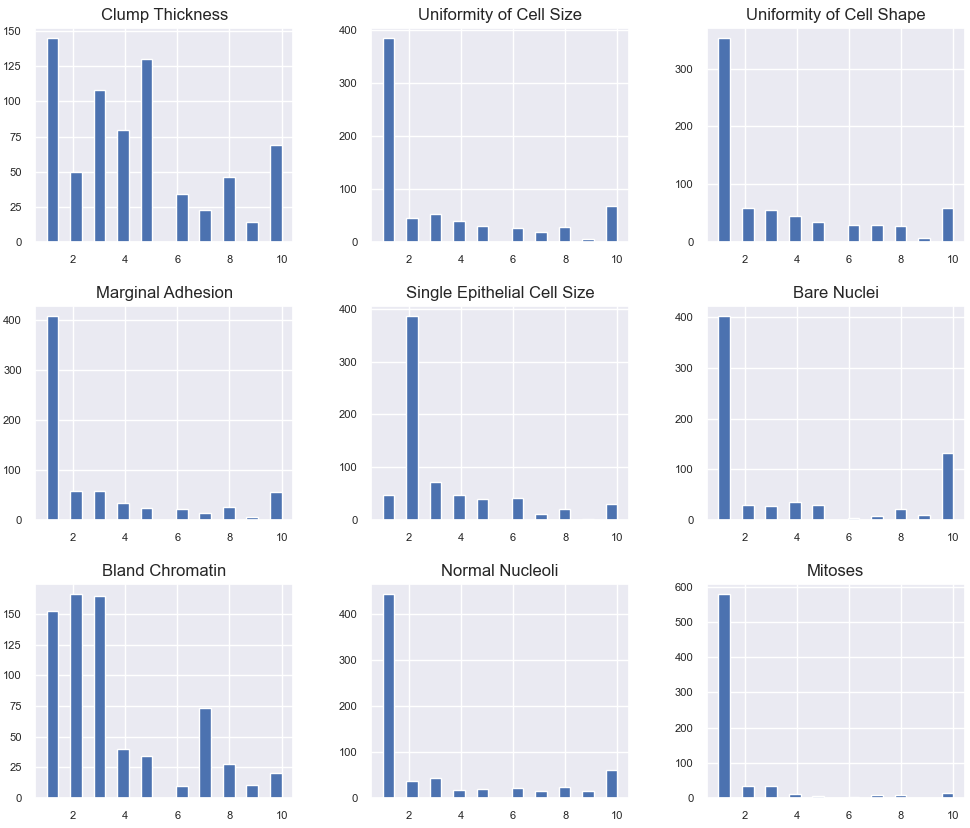
\includegraphics[width=0.75\textwidth]{res3/hist1.png}
%	\caption{样本直方图}
%	\label{fig:hist1}
%\end{figure}
\begin{figure}[H]
	\centering
	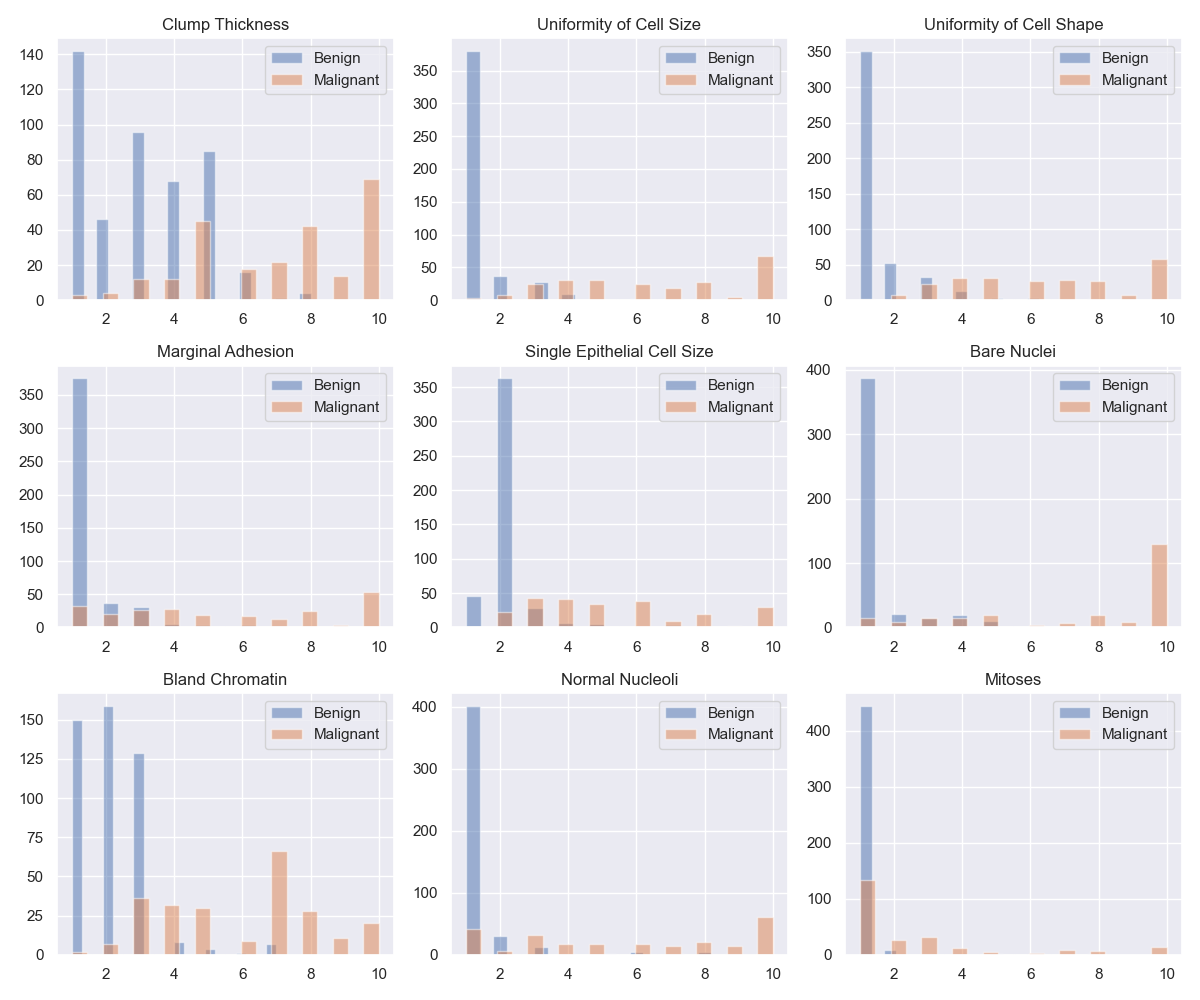
\includegraphics[width=0.8\textwidth]{res3/hist2.png}
	\caption{按照Class分类的样本直方图}
	\label{fig:hist2}
\end{figure}
由上述直方图可看出,肿瘤块状厚度为1的数量最多,且根据条状颜色分布可知,良性肿瘤的块状厚度偏小,而恶行肿瘤的块状厚度偏大;肿瘤细胞大小均匀性为1的数量最多,细胞大小为2—10的数量几乎相等。且根据条状颜色分布可知,良性肿瘤的细胞大小的均匀性集中分布于1,而恶性肿瘤的细胞大小均匀性几乎均匀分布于3-10;观察其他特征的分布可发现,其与上述特征的分布近似相同,总结来看,良性肿瘤的特征均偏低,且分布集中,而恶性肿瘤的特征偏低,且分布近似均匀。且从样本平衡性来看,除肿瘤块状厚度的样本分布较为均匀外,其余特征的样本分布集中分布于取值较低的特征处,且良性肿瘤样本数远大于恶性肿瘤样本数,即样本均衡性较差。\par 
\begin{figure}[H]
	\centering
	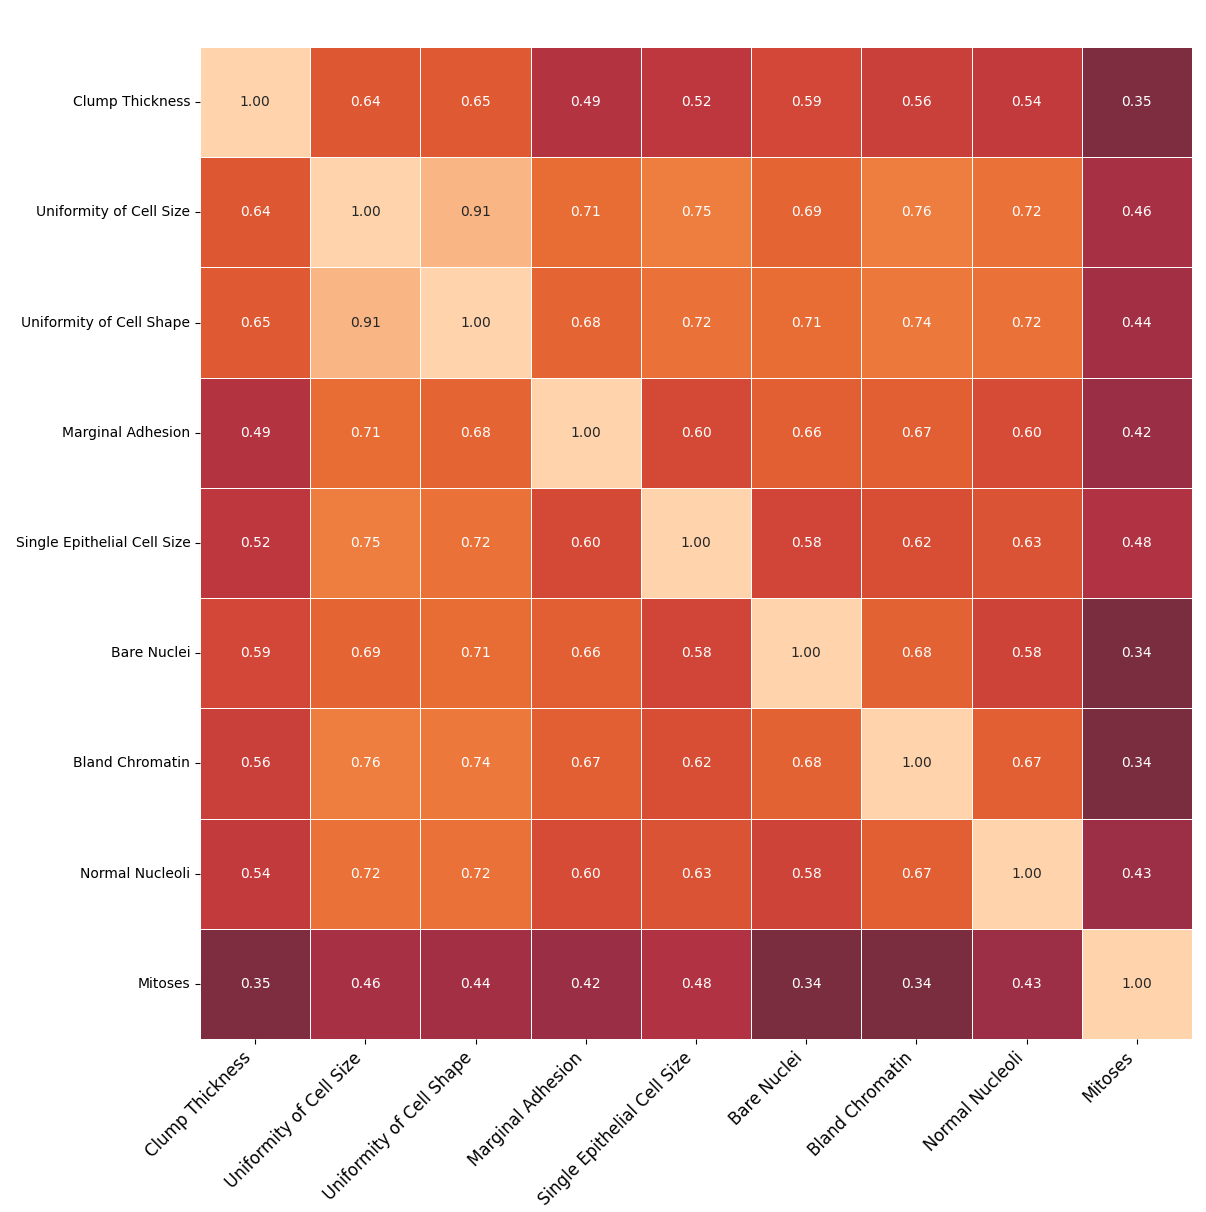
\includegraphics[width=0.9\textwidth]{res3/heatmap.png}
	\caption{相关性热力图}
	\label{fig:heatmap}
\end{figure}
分析九个自变量的相关性情况,如图\ref{fig:heatmap}所示。可以观察到,自变量之间的相关性比较高。
\clearpage
\subsection{评价指标}
在这一部分中,主要对所选择的模型评价标准参数进行说明。本次共选择五种评价标准进行评价,分别为 Precision、Recall、F1-Score、Maro Avg 和 Weighted Avg。分类器的预测结果可以分为四种情况:
\begin{enumerate}
	\item 真正例(True Positive,TP):分类器将一个实际为正例的样本正确地预测为正例。
	\item 真反例(True Negative,TN):分类器将一个实际为反例的样本正确地预测为反例。
	\item 假正例(False Positive,FP):分类器将一个实际为反例的样本错误地预测为正例。
	\item 假反例(False Negative,FN):分类器将一个实际为正例的样本错误地预测为反例。
\end{enumerate}

精确率 Precision 表示分类器预测为正例的样本中有多少是真正例,定义为
\begin{equation*}
	Precision = \frac{TP}{TP + FP}
\end{equation*}
\par 召回率 Recall 表示真正例中有多少被分类器正确地预测出来了,定义为
\begin{equation*}
	Recall = \frac{TP}{TP + FN}
\end{equation*}
\par 二者的区别在于精确率的分母是预测到的正类,它的提出是让模型的现有预测结果尽可能不出错,即宁愿漏检,也不能让现有的预测有错。而召回率的分母是原本的正类,它的提出是让模型预测到所有想被预测到的样本,即就算多预测一些错的,也能接受。\par
F1-Score 综合了精确率和召回率,是二者的调和平均数,定义为
\begin{equation*}
	\text{F1-Score} = 2\cdot\frac{Precision\times Recall}{Precision+Recall} = \frac{TP}{TP+\frac{1}{2}(FP+FN)}
\end{equation*}
宏平均 Maro Avg 定义为 benign 和 malignant 的 Precision 或 Recall 或 F1-Score 的算数平均值。加权平均 Weighted Avg 的定义为用每一个类别(benign和malignant)的样本数量在所有类别的样本总数的占比作为权重,然后计算 Precision 或 Recall 或 F1-Score 的加权平均值。
\clearpage
\section{线性判别分类}
\subsection{基本原理}
线性判别分类(Linear Discriminant Analysis,LDA)是一种经典的线性分类方法,它假设不同类别的数据是从不同的高斯分布中生成的,并寻找一个投影方向,将数据投影到一条直线上,使得同类样本的投影点尽可能接近,不同类样本的投影点尽可能远离。在投影后的低维空间中,可以使用一个线性分类器进行分类。\par 
设有 $K$ 个类别,每个类别的样本在 $n$ 维特征空间中服从均值向量为 $\boldsymbol{\mu}_k$,协方差矩阵为 $\boldsymbol{\Sigma}$ 的高斯分布。则对于一个新样本 $\mathbf{x}$,LDA 将它投影到一条直线上,使得同类样本的投影点尽可能接近,不同类样本的投影点尽可能远离,即通过最大化下面的目标函数来确定投影方向 $\mathbf{w}$:
$$
J(\mathbf{w})=\frac{\mathbf{w}^\top\mathbf{S}_B\mathbf{w}}{\mathbf{w}^\top\mathbf{S}_W\mathbf{w}}
$$
其中,$\mathbf{S}_B$ 是类间散度矩阵,$\mathbf{S}_W$ 是类内散度矩阵,定义为:
$$\begin{aligned}
	\mathbf{S}_B &= \sum_{k=1}^{K}N_k(\boldsymbol{\mu}_k - \boldsymbol{\mu})(\boldsymbol{\mu}_k - \boldsymbol{\mu})^\top \\
	\mathbf{S}_W &= \sum_{k=1}^{K}\sum_{\mathbf{x}_i\in D_k}(\mathbf{x}_i - \boldsymbol{\mu}_k)(\mathbf{x}_i - \boldsymbol{\mu}_k)^\top
\end{aligned}$$
其中,$N_k$ 表示属于类别 $k$ 的样本数量,$D_k$ 表示属于类别 $k$ 的样本集合,$\boldsymbol{\mu}$ 是所有样本的均值向量。\par 
解出最优的投影方向 $\mathbf{w}$ 后,对于一个新的样本 $\mathbf{x}$,将其投影到直线上得到一个标量 $z=\mathbf{w}^\top\mathbf{x}$,然后使用阈值将其分类到不同的类别。\par 
LDA 的主要优点是在样本数量比较少、特征维度较高的情况下仍然能够获得较好的分类效果,缺点是假设数据服从高斯分布,并且需要计算类别内协方差矩阵的逆矩阵,当特征维度较高时,计算量会很大。
\subsection{数值实验}
使用 LDA 方法对样本进行分类,如下所示。输出的分类准确率为 95.71\%,混淆矩阵如图\ref{fig:lda}所示。表\ref{tbl:lda}展示了 LDA 分类器的性能。\par 
\lstset{language=Python}
\lstset{frame=lines}
\lstset{caption={LDA 分类}}
\lstset{label={lst:code_direct}}
\lstset{basicstyle=\footnotesize}
\begin{lstlisting}
	lda = LinearDiscriminantAnalysis()
	cross_val_model(lda)
\end{lstlisting}
\begin{figure}[H]
	\centering
	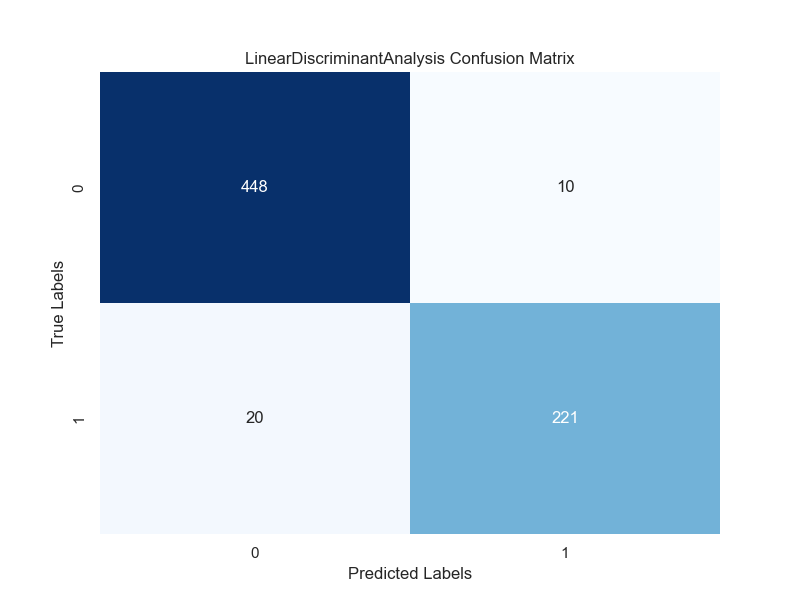
\includegraphics[width=0.9\textwidth]{res3/lda.png}
	\caption{LDA 分类混淆矩阵}
	\label{fig:lda}
\end{figure}
\begin{table}[H]
	\centering
	\begin{tabular}{lccc}
		\toprule
		\textbf{Class} & \textbf{Precision} & \textbf{Recall} & \textbf{F1-Score} \\
		\midrule
		\textbf{benign} & 0.96 & 0.98 & 0.97 \\
		\textbf{malignant} & 0.96 & 0.918 & 0.938 \\
		\midrule
		\textbf{Macro Avg} & 0.958 & 0.948 & 0.952 \\
		\textbf{Weighted Avg} & 0.97 & 0.958 & 0.958 \\
		\bottomrule
	\end{tabular}
	\caption{LDA 分类器性能}
	\label{tbl:lda}
\end{table}
对于良性类别,分类器的 precision 和 recall 指标都非常高,分别为 0.96 和 0.98,这意味着分类器在识别良性肿瘤细胞时非常准确且有很好的召回率。对于恶性类别,分类器的 precision 指标也很高,为 0.96,但是 recall 指标相对较低,为 0.918,这意味着分类器在预测恶性肿瘤细胞时准确性较低。不过,该类别的 f1-score 指标仍然较高,为0.938。

\clearpage
\section{Logistic回归}
\subsection{基本原理}
Logistic 回归(Logistic Regression)是一种用于二分类问题的机器学习算法,它基于对数据的线性拟合和 Logistic 函数的映射来估计概率。具体来说,Logistic 回归模型假设输出变量 $y$ 的条件概率分布为 $P(y=1|\mathbf{x})=\sigma(\mathbf{w}^\top \mathbf{x}+b)$,其中 $\sigma(\cdot)$ 是Logistic函数(sigmoid函数),$\mathbf{x}$ 是输入特征向量,$\mathbf{w}$ 和 $b$ 是模型参数。Logistic 函数将线性函数的输出转换为一个取值在 $[0, 1]$ 区间的概率值,因此模型可以输出输入为 $\mathbf{x}$ 时 $y=1$ 的概率,也可以输出 $y=0$ 的概率 $P(y=0|\mathbf{x})=1-P(y=1|\mathbf{x})$。\par 

在 Logistic 回归中,模型参数 $\mathbf{w}$ 和 $b$ 通过最大化训练数据的似然函数来学习,似然函数表示为:
\begin{equation*}
	L(\mathbf{w},b) = \prod_{i=1}^n P(y_i|\mathbf{x}_i;\mathbf{w},b) = \prod_{i=1}^n [\sigma(\mathbf{w}^\top \mathbf{x}_i+b)]^{y_i}[1-\sigma(\mathbf{w}^\top \mathbf{x}_i+b)]^{1-y_i}
\end{equation*}
其中,$n$ 是训练样本的数量,$y_i$ 是样本 $\mathbf{x}_i$ 对应的标签。为了避免过拟合,通常还会对似然函数加入一个正则化项,形式为 $\frac{\lambda}{2}|\mathbf{w}|^2$,其中 $\lambda$ 是正则化系数。最终的目标是最大化似然函数和正则化项的和,即
\begin{equation*}
	\max_{\mathbf{w},b} L(\mathbf{w},b) - \frac{\lambda}{2}\|\mathbf{w}\|^2
\end{equation*}
通常使用梯度下降等优化算法来求解上述优化问题,从而得到最优的参数 $\mathbf{w}$ 和 $b$。Logistic 函数的形式为:
\begin{equation*}
	\sigma(z) = \frac{1}{1+\exp(-z)}
\end{equation*}
其中,$z=\mathbf{w}^\top \mathbf{x}+b$。\par 
Logistic 回归模型用于二分类的原理为:当 $z$ 很大时,$\sigma(z)$ 接近于 $1$,即 $y=1$ 的概率很高;当 $z$ 很小时,$\sigma(z)$ 接近于 $0$,即 $y=0$ 的概率很高。
\subsection{数值实验}
使用 Logistic 回归方法对样本进行分类,如下所示。
\lstset{language=Python}
\lstset{frame=lines}
\lstset{caption={Logistic 回归}}
\lstset{label={lst:code_direct}}
\lstset{basicstyle=\footnotesize}
\begin{lstlisting}
	lr = LogisticRegression()
	cross_val_model(lr)
\end{lstlisting}
输出的分类准确率为 96.14\%,混淆矩阵如图\ref{fig:logistic}所示。表\ref{tbl:logistic}展示了 Logistic 回归分类器的性能。可以看出,Logistic 回归方法的分类效果和 LDA 方法效果相近。
\begin{figure}[h]
	\centering
	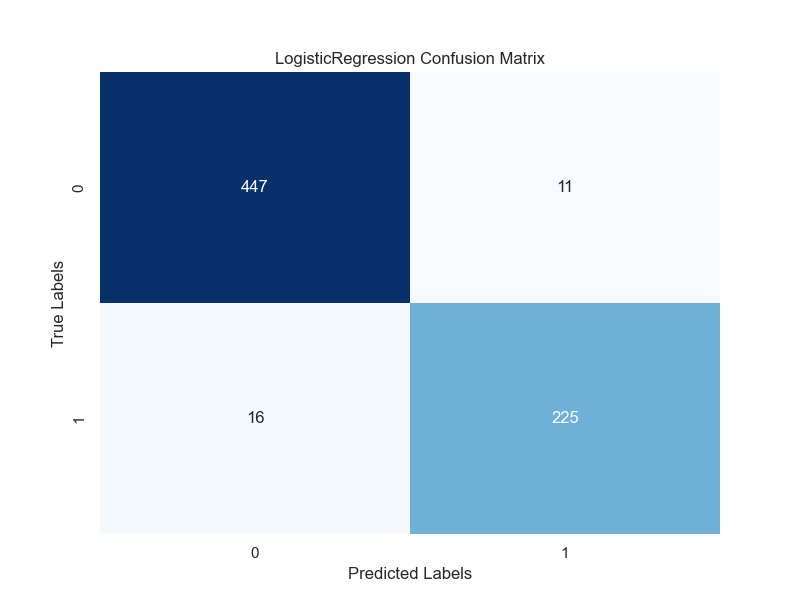
\includegraphics[width=0.9\textwidth]{res3/logistic.png}
	\caption{Logistic 回归混淆矩阵}
	\label{fig:logistic}
\end{figure}
\begin{table}[h]
	\centering
	\begin{tabular}{lccc}
		\toprule
		\textbf{Class} & \textbf{Precision} & \textbf{Recall} & \textbf{F1-Score} \\
		\midrule
		\textbf{benign} & 0.97 & 0.975 & 0.971 \\
		\textbf{malignant} & 0.95 & 0.938 & 0.943 \\
		\midrule
		\textbf{Macro Avg} & 0.96 & 0.955 & 0.955 \\
		\textbf{Weighted Avg} & 0.96 & 0.96 & 0.961 \\
		\bottomrule
	\end{tabular}
	\caption{Logistic 回归分类器性能}
	\label{tbl:logistic}
\end{table}


\clearpage
\section{K最近邻分类}
\subsection{基本原理}
K最近邻(K-Nearest Neighbor,KNN)分类器是一种基于实例的监督学习算法。它的基本原理是根据样本间的距离度量,通过查找与测试样本最近的K个训练样本,来预测测试样本的类别。\par 
KNN算法的核心是距离度量,常见的距离度量有欧氏距离、曼哈顿距离、闵可夫斯基距离等。以欧氏距离为例,如果训练集中的某个样本的特征向量为$x_i$,测试样本的特征向量为$x$,则它们之间的欧氏距离为: 
\begin{equation*}
	d_{i}=\sqrt{\sum_{j=1}^{m}\left(x_{i, j}-x_{j}\right)^{2}}
\end{equation*}
其中,$m$表示特征的数量。\par 
当测试样本的欧氏距离与训练样本的欧氏距离都计算完毕后,KNN算法会选出距离测试样本最近的K个训练样本,并将它们的类别进行统计。通常采用多数表决的方式,即把这K个训练样本中出现次数最多的类别作为测试样本的类别输出。
\subsection{数值实验}
\subsubsection{确定最佳k值}
由下所示,通过穷举法寻找最佳K值。输出结果为K=9.
\lstset{language=Python}
\lstset{frame=lines}
\lstset{caption={KNN 回归}}
\lstset{label={lst:code_direct}}
\lstset{basicstyle=\footnotesize}
\begin{lstlisting}
	scores = []
	for k in range(1, 31):
		knn = KNeighborsClassifier(n_neighbors=k)
		score = cross_val_score(knn, X_train, y_train, cv=5).mean()
		scores.append(score)
	
	best_k = np.argmax(scores) + 1
	print(f'Best k:{best_k}')  # Best k:9
\end{lstlisting}
\subsubsection{使用K=9的KNN分类器进行分类}
输出的分类准确率为96.42\%,混淆矩阵如图\ref{fig:knn}所示。表\ref{tbl:knn}展示了KNN分类器的性能。\par 
\begin{figure}[H]
	\centering
	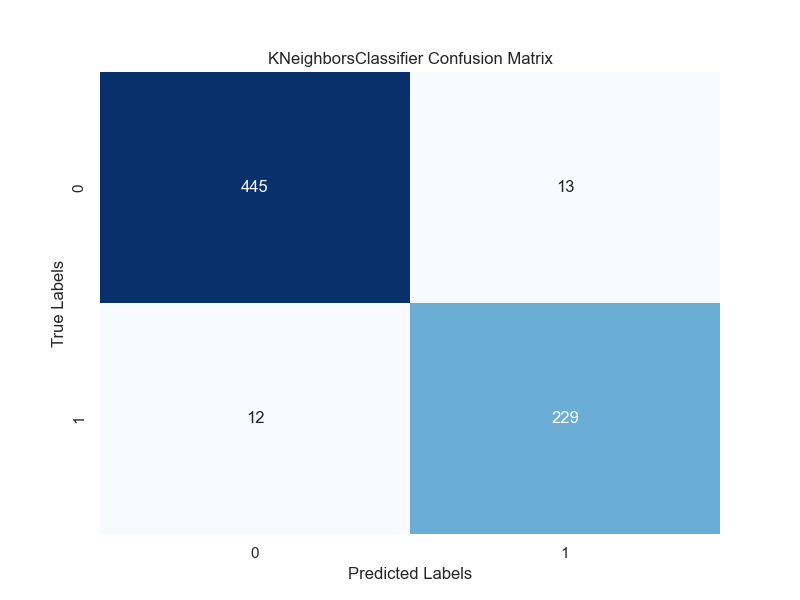
\includegraphics[width=0.9\textwidth]{res3/knn.png}
	\caption{KNN 分类混淆矩阵}
	\label{fig:knn}
\end{figure}
\begin{table}[H]
	\centering
	\begin{tabular}{lccc}
		\toprule
		\textbf{Class} & \textbf{Precision} & \textbf{Recall} & \textbf{F1-Score} \\
		\midrule
		\textbf{benign} & 0.976 & 0.974 & 0.972 \\
		\textbf{malignant} & 0.948 & 0.95 & 0.948 \\
		\midrule
		\textbf{Macro Avg} & 0.958 & 0.96 & 0.962 \\
		\textbf{Weighted Avg} & 0.962 & 0.962 & 0.962 \\
		\bottomrule
	\end{tabular}
	\caption{KNN 分类器性能}
	\label{tbl:knn}
\end{table}
可以看出,Precision、Recall和F1-Score都很高。针对恶性类别,Precision、Recall和F1-Score指标都略低于良性类别,分别为0.948、0.95和0.948。这意味着分类器在识别恶性样本时,可能存在将其错误地分类为良性的情况。但总体来说,分类器在分类任务中表现良好。
\clearpage
\section{朴素贝叶斯分类}
\subsection{基本原理}
\subsubsection{朴素贝叶斯分类}
	朴素贝叶斯分类是一种基于贝叶斯定理的分类方法,它假设不同特征之间相互独立,从而简化了模型的计算和训练。该方法广泛应用于自然语言处理、文本分类、垃圾邮件过滤等领域。\par 
	假设我们有一个包含 $n$ 个样本的数据集 $D = {(x_1, y_1), (x_2, y_2), ..., (x_n, y_n)}$,其中 $x_i$ 表示第 $i$ 个样本的特征,$y_i$ 表示第 $i$ 个样本的标签。假设每个样本有 $m$ 个特征,我们需要根据这些特征预测样本所属的类别,即 $P(y|x)$,其中 $y$ 表示类别,$x$ 表示特征。\par 

	朴素贝叶斯分类的核心思想是根据贝叶斯定理计算后验概率 $P(y|x)$,即样本 $x$ 属于类别 $y$ 的概率。根据贝叶斯定理,后验概率可以表示为:
	\begin{equation}\label{eq:hygl}
	P(y|x) = \frac{P(x|y)P(y)}{P(x)}
	\end{equation}
	其中 $P(x|y)$ 表示在给定类别 $y$ 的情况下样本 $x$ 出现的概率,$P(y)$ 表示类别 $y$ 在样本集中出现的概率,$P(x)$ 表示样本 $x$ 出现的概率。\par

	由于我们要比较不同类别的后验概率,因此可以忽略分母 $P(x)$。又因为朴素贝叶斯算法假设每个特征之间相互独立,因此可以将 $P(x|y)$ 表示为每个特征的条件概率的乘积:
	\begin{equation}\label{eq:tjglcj}
	P(x|y) = P(x_1, x_2, ..., x_m | y) = \prod_{i=1}^{m}P(x_i|y)
	\end{equation}
	综合(\ref{eq:hygl})(\ref{eq:tjglcj})两式,我们得到后验概率的计算公式:
	\begin{equation*}
		P(y|x) = \frac{P(y)\prod_{i=1}^{m}P(x_i|y)}{P(x)}
	\end{equation*}
	其中 $P(x_i | y)$ 表示在给定类别 $y$ 的情况下,特征 $x_i$ 出现的概率。在朴素贝叶斯分类中,$P(x_i | y)$ 可以根据训练集中类别 $y$ 和特征 $x_i$ 的出现频率来估计。常见的估计方法有极大似然估计和贝叶斯估计等。最终,我们将选择使得 $P(y|x)$ 最大的类别作为样本 $x$ 的预测类别:
	\begin{equation}\label{eq:bayes}
		\hat{y} = \text{arg}\max_{y\in Y}P(y|x)=\text{arg}\max_{y\in Y}P(y)\prod_{i=1}^{m}P(x_i|y)
	\end{equation}
	其中 $\hat{y}$ 表示样本 $x$ 的预测类别,$Y$ 表示所有可能的类别。
\subsubsection{朴素贝叶斯分类器}
	朴素贝叶斯分类器是基于贝叶斯定理和特征独立假设的一类分类算法,常用于文本分类、垃圾邮件过滤、情感分析等任务中。根据先验分布的不同,即对公式(\ref{eq:bayes})中 $P(x_i|y)$ 处理的不同,朴素贝叶斯分类器可以分为以下三种常用的分类器。
	\paragraph{伯努利朴素贝叶斯分类器(Bernoulli Naive Bayes)}
	伯努利朴素贝叶斯分类器适用于二元离散特征的分类问题。它假设每个特征的取值只有 0 和 1 两种,即特征是布尔型的。伯努利朴素贝叶斯的决策规则为:
	\begin{equation*}
		P(x_i|y) = \left\{ 
		\begin{array}{ll}
				P(x_i=1|y), &\quad x_i = 1 \\
				1 - P(x_i=1|y), &\quad x_i = 0 
		\end{array} \right.
	\end{equation*}
	\paragraph{多项式朴素贝叶斯分类器(Multinomial Naive Bayes)}
	多项式朴素贝叶斯分类器适用于多元离散特征的分类问题。它假设每个特征的取值为一个离散的计数值,即特征是计数型的。在多项式朴素贝叶斯分类器中,分布由每个类 $y$ 的向量 $\theta_y = (\theta_{y1}, ..., \theta_{yn})$ 参数化,其中 $n$ 是特征数,$\theta_{yi}$ 就是特征 $i$ 出现在属于 $y$ 类的样本中的概率 $P(x_i|y)$。参数 $\theta_y$ 可以通过极大似然估计来计算得到:
	\begin{equation}\label{eq:multi}
		\hat{\theta_{yi}} = \frac{N_{yi}+\alpha_i}{N_{y}+\alpha}
	\end{equation}
	其中 $N_{yi}$ 表示在训练集中样本属于 $y$ 这个类别下特征 $i$ 出现的频次。即 $N_{yi} = \sum_{x\in T} x_i$;$N_y$ 表示类别 $y$ 下所有特征的总频次,即 $N_y = \sum_{i=1}^{n} N_{yi}$;$\alpha_i$ 表示每个特征维度对应的平滑系数,$\alpha$表示所有平滑系数的总和。\par 
	在实际处理时,每个维度的平滑系数一般被设为相等,因此式(\ref{eq:multi})可以写为:
	\begin{equation}\label{eq:multi2}
		\hat{\theta_{yi}} = \frac{N_{yi}+\alpha}{N_{y}+\alpha n}
	\end{equation}
	在这里,$\alpha$ 表示的是每个特征维度的平滑系数。根据公式(\ref{eq:multi2})估计得到类别下各个特征的条件概率后,便可以通过公式(\ref{eq:bayes})来最大化后验概率,以此确定样本的分类类别。
	\paragraph{高斯朴素贝叶斯分类器(Gaussian Naive Bayes)}
	高斯朴素贝叶斯分类器适用于连续型特征的分类问题。它假设每个特征的取值都服从高斯分布(正态分布),即特征是连续型的。在高斯朴素贝叶斯分类器中,条件概率 $P(x_i | y)$ 通常采用高斯分布进行估计,即:
	$$ P(x_i|y) = \frac{1}{\sqrt{2\pi\sigma_y^2}}\exp\left(-\frac{(x_i-\mu_y)^2}{2\sigma_y^2}\right) $$
	其中 $\mu_y$ 和 $\sigma_y^2$ 分别是训练集中所有属于类别 $y$ 的样本在第 $i$ 个特征上的均值和方差。在计算得到每个特征维度的条件概率后,再进行极大化后验概率计算。\par 
	对于我们的乳腺癌数据集来说,比较适合的分类器是高斯朴素贝叶斯分类器和多项式朴素贝叶斯分类器。考虑高斯朴素贝叶斯分类器,我们可以认为数据集中样本除去id外的的9个特征是连续型的,即使它们只在0-10之间取整数;考虑多项式朴素贝叶斯分类器,特征本就是计数型的,即使从意义上并非如此。该数据集不适用于伯努利朴素贝叶斯分类器,它要求每个特征值,即x的取值,只有0和1两种,而该数据集的特征值并不符合。
\subsection{数值实验}
\subsubsection{高斯朴素贝叶斯分类器}
使用高斯朴素贝叶斯分类器对样本进行分类,如下所示。
\lstset{language=Python}
\lstset{frame=lines}
\lstset{caption={高斯朴素贝叶斯}}
\lstset{label={lst:code_direct}}
\lstset{basicstyle=\footnotesize}
\begin{lstlisting}
	nb = GaussianNB()
	cross_val_model(nb)
\end{lstlisting}
输出的分类准确率为 95.99\%,混淆矩阵如图\ref{fig:gaussnb}所示。表\ref{tbl:gaussnb}展示了高斯朴素贝叶斯分类器的性能。\par 
\begin{figure}[h]
	\centering
	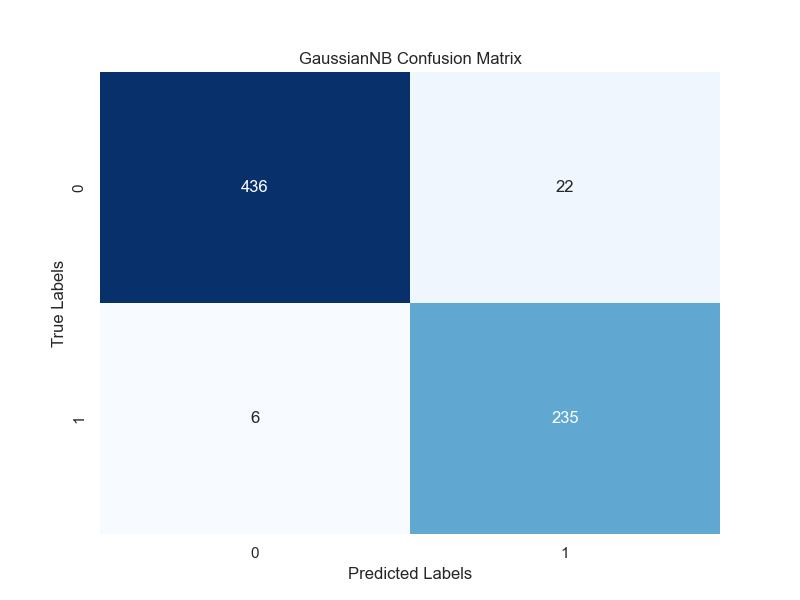
\includegraphics[width=0.9\textwidth]{res3/gaussiannb.png}
	\caption{高斯朴素贝叶斯分类器混淆矩阵}
	\label{fig:gaussnb}
\end{figure}
\begin{table}[H]
	\centering
	\begin{tabular}{lccc}
		\toprule
		\textbf{Class} & \textbf{Precision} & \textbf{Recall} & \textbf{F1-Score} \\
		\midrule
		\textbf{benign} & 0.988 & 0.954 & 0.968 \\
		\textbf{malignant} & 0.916 & 0.976 & 0.944 \\
		\midrule
		\textbf{Macro Avg} & 0.95 & 0.964 & 0.956 \\
		\textbf{Weighted Avg} & 0.964 & 0.958 & 0.958 \\
		\bottomrule
	\end{tabular}
	\caption{高斯朴素贝叶斯分类器性能}
	\label{tbl:gaussnb}
\end{table}
可以注意到 precision、recall 和 f1-score 都很高。针对恶性类别,precision、recall 和 f1-score 指标都略低于良性类别,分别为 0.916、0.976 和 0.944。这意味着分类器在识别恶性样本时,可能存在将其错误地分类为良性的情况。但总体来说,分类器在分类任务中表现良好。
\subsubsection{多项式朴素贝叶斯分类器}\label{6.2.2}
改用多项式朴素贝叶斯分类器如下所示。
\lstset{language=Python}
\lstset{frame=lines}
\lstset{caption={多项式朴素贝叶斯}}
\lstset{label={lst:code_direct}}
\lstset{basicstyle=\footnotesize}
\begin{lstlisting}
	nb3 = MultinomialNB(alpha=1.0e-10, force_alpha=True)
	cross_val_model(nb3)
\end{lstlisting}
输出的分类准确率为88.84\%,混淆矩阵如图\ref{fig:multinb}所示。\par 
\begin{figure}[h]
	\centering
	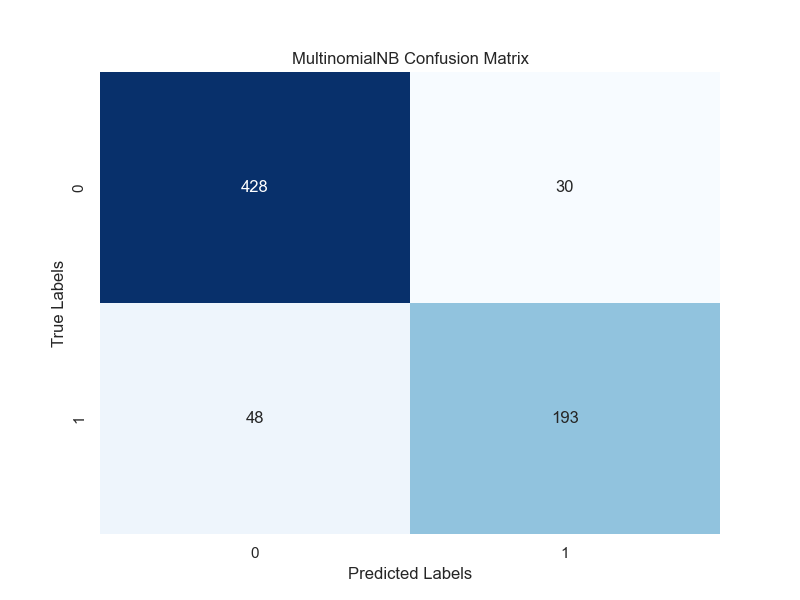
\includegraphics[width=0.9\textwidth]{res3/multinomialnb.png}
	\caption{多项式朴素分类器混淆矩阵}
	\label{fig:multinb}
\end{figure}
经计算,precision 为 0.865,recall 为 0.801,f1-score 为 0.832。与高斯朴素贝叶斯分类器相比,多项式贝叶斯分类器在威斯康星乳腺癌数据集上的表现显然更差。可能的原因之一是多项式贝叶斯分类器假设特征之间是相互独立的,在威斯康星乳腺癌数据集中,特征之间存在较强的相关性,如图\ref{fig:heatmap}所示。这可能导致了分类器的性能下降。另外,与高斯朴素贝叶斯分类器相比,多项式贝叶斯分类器通常更适用于文本分类等具有大量离散特征的任务。在威斯康星乳腺癌数据集上,特征维度相对较低,这可能也是性能下降的原因之一。
\subsubsection{拉普拉斯平滑}\label{6.2.3}
拉普拉斯平滑是一种平滑技术,常用于解决概率模型中的零概率问题。该方法通过给计数值添加一个正的常数 $\alpha$(通常为1),来避免出现零概率的情况。对于一个概率模型,拉普拉斯平滑可以通过以下公式来计算未出现事件的概率:
\begin{equation*}
	P(x_i) = \frac{count(x_i) + 1}{N + |X|}
\end{equation*}
其中,$count(x_i)$ 表示 $x_i$ 出现的次数,$N$ 表示总的样本数,$|X|$ 表示样本空间中不同的取值个数。因此,对于任何一个未出现的事件,它的计数值为 0,通过拉普拉斯平滑,可以使其概率为 $\frac{1}{N + |X|}$,从而避免了零概率问题的出现。\par 
在高斯朴素贝叶斯分类器中,由于假设每个特征的取值都服从正态分布,故事件发生的概率 $P(x_i)$ 不可能为0,因此不适用拉普拉斯平滑。对多项式朴素贝叶斯分类器使用拉普拉斯平滑(即 $\alpha=1$)。\par 
在实际操作中,我们发现使用拉普拉斯平滑的效果受随机种子数影响非常大,即受训练集和测试集的划分方法的影响非常大,故在5折交叉验证中选择随机种子数 0-999。打印极差,发现极差为 0.7\%。这意味着拉普拉斯平滑对分类几乎不产生影响。代码运行过程中无警告,这表示在这 1000 次实验中,nb3 模型没有出现零概率的情况。
\vspace{\baselineskip}
\lstset{language=Python}
\lstset{frame=lines}
\lstset{caption={拉普拉斯平滑}}
\lstset{label={lst:code_direct}}
\lstset{basicstyle=\footnotesize}
\begin{lstlisting}
	nb3 = MultinomialNB(alpha=0, force_alpha=True)
	nb4 = MultinomialNB(alpha=1)
	lst_accuracy = []
	
	for i in range(1000):
		accuracy3 = cross_val_model2(nb3, i)
		accuracy4 = cross_val_model2(nb4, i)
	
		if accuracy3 != accuracy4:
			lst_accuracy.append(accuracy4-accuracy3)
	
	print(max(lst_accuracy)-min(lst_accuracy))
\end{lstlisting}
% 可能的原因:
% 1. 对于每个属性,每个类的实例够多(但由直方图看,并不是这么回事。和划分数据集的随机种子数也没关系啊,用另一个模型种子数42就显示出现零概率。)
% 2. 对于本数据集,良性肿瘤的特征比较集中。

\vspace{3\baselineskip}
\section{比较分析}
根据参数说明中的五种办法,首先对利用高斯朴素贝叶斯分类器和多项式朴素贝叶斯分类器的分类结果进行比较,得出对于本次数据的最优朴素贝叶斯分类器,然后再将其和线性判别、Logistic回归、KNN分类得出的数据结果进行比较分析,得出最适合本次数据的最优分类方法。\par 
由\ref{6.2.3}结果可知,对于本次数据,拉普拉斯平滑前后的分类效果并无显著差异,所以我们仍选择用拉普拉斯平滑前的分类器所得结果进行比较。\par 
在\ref{6.2.2}中,根据高斯朴素贝叶斯分类器和多项式朴素贝叶斯分类器的Precision、Recall、F1-Score可知,高斯朴素贝叶斯分类器的分类效果更优,所以选择高斯朴素贝叶斯分类器为本次数据的最优朴素贝叶斯分类器。\par 
下面对四种分类方法的结果进行比较分析。
\begin{table}[H]
	\centering
	\caption{四种分类方法的Precision、Recall、F1-Score结果}
	\label{tab:analysis1}
	\begin{tblr}{
			cells = {c},
			cell{2}{1} = {r=2}{},
			cell{4}{1} = {r=2}{},
			cell{6}{1} = {r=2}{},
			vline{2-6} = {1-7}{},
			hline{1,2,8} = {-}{0.08em},
			hline{2,4,6} = {-}{},
		}
		& 类别        & 线性判别  & Logistic回归 & KNN分类 & 高斯朴素贝叶斯分类 \\
		Precision & Benign    & 0.96  & 0.97       & 0.976 & 0.988     \\
		& Malignant & 0.96  & 0.95       & 0.948 & 0.916     \\
		Recall    & Benign    & 0.98  & 0.975      & 0.974 & 0.954     \\
		& Malignant & 0.918 & 0.938      & 0.95  & 0.976     \\
		F1-Score  & Benign    & 0.97  & 0.971      & 0.972 & 0.968     \\
		& Malignant & 0.938 & 0.943      & 0.948 & 0.944     
	\end{tblr}
\end{table}
由表\ref{tab:analysis1}可知,对于良性肿瘤(Benign)而言,高斯朴素贝叶斯分类器的 Precision 最高,线性判别的 Recall 最高,KNN 分类的 F1-Score 最高,对于恶性肿瘤(Malignant)而言,线性判别的 Precision 最高,高斯朴素贝叶斯分类的 Recall 最高,KNN 分类的 F1-Score 最高。但在实际情况中,我们有时可能无法已知肿瘤是良性还是恶性的,所以选择 Macro Avg 和 Weighted Avg 这两种评价标准对四种分类方法进行综合评价。
\begin{table}[H]
	\centering
	\caption{四种分类方法的Macro Avg、Weighted Avg结果}
	\label{tab:analysis2}
	\begin{tblr}{
			cells = {c},
			cell{2}{1} = {r=3}{},
			cell{5}{1} = {r=3}{},
			vline{2-6} = {1-7}{},
			hline{1,2,8} = {-}{0.08em},
			hline{5} = {-}{},
		}
		& 评价指标      & 线性判别  & Logistic回归 & KNN分类 & 高斯朴素贝叶斯分类器 \\
		Macro Avg    & Precision & 0.958 & 0.96       & 0.958 & 0.95       \\
		& Recall    & 0.948 & 0.955      & 0.96  & 0.964      \\
		& F1-Score  & 0.952 & 0.955      & 0.962 & 0.956      \\
		Weighted Avg & Precision & 0.97  & 0.96       & 0.962 & 0.964      \\
		& Recall    & 0.958 & 0.96       & 0.962 & 0.958      \\
		& F1-Score  & 0.958 & 0.961      & 0.962 & 0.958      
	\end{tblr}
\end{table}
由表\ref{tab:analysis2}易知,选择 Macro Avg 和 Weighted Avg 这两种评价标准会选择出不同的最优分类方法。根据定义,Macro Avg 是一种算术平均的评价标准,而 Weighted Avg 是加权平均,它充分考虑了样本中良性肿瘤和恶性肿瘤样本数不同所带来的影响,所以选择 Weighted Avg 更加科学。对于 Weighted Avg 评价标准,线性判别的 Precision 最高,KNN 分类的 Recall 和 F1-Score 最高。\par 
根据评价标准的定义并结合实际情况,对于本数据来说,若需要最综合的分类结果,KNN 分类的效果最佳;若想尽可能提高肿瘤预测的准确率,线性判别的效果最佳;若想尽可能提高良性肿瘤预测的准确率,高斯朴素贝叶斯分类的效果最佳;若想尽可能提高恶性肿瘤预测的准确率,线性判别的效果最佳;若想尽可能把所有恶性肿瘤都预测到,高斯朴素贝叶斯分类的效果最佳。
\vspace{-\baselineskip}
\section{总结与反思}
在此论文中我们运用logistic回归、线性判别分析、knn分类与朴素贝叶斯算法四种算法实现对肿瘤类型的预测。通过对比分析可知knn算法实现分类的效果最优、最稳定。其中朴素贝叶斯算法中使用高斯朴素贝叶斯分类器的优于多项式朴素贝叶斯分类器效果。\par 
但在实现算法的过程中也发现了部分问题,因此进行反思如下:
\begin{enumerate}
	\item 由四种算法预测效果的对比知,良性肿瘤的预测效果均优于恶性肿瘤的预测效果,对于上述结果,我们组进行讨论反思认为,这与样本不均衡性有很大关系。在描述性统计分析即可知本数据集的良性肿瘤与恶性肿瘤数据分布较为不均,且以良性肿瘤样本数量居多。因良性肿瘤样本数据多而提供的信息较恶性肿瘤丰富,所以预测效果较好。另外,良性肿瘤的各特征取值均偏低且集中,而恶性肿瘤的各特征取值较为分散均匀。因此当特征取值较低时我们趋向于认为其属于良性肿瘤类别,即特征对良性肿瘤的识别度较高,因此对良性肿瘤的预测效果较好。
	\item 由数据预处理发现部分特征之间存在较强的相关性,而朴素贝叶斯算法建立要求特征满足条件独立。因此特征之间较强相关性可能是导致朴素贝叶斯算法预测效果较差的重要原因。
\end{enumerate}
	
\end{document}